\documentclass[10pt]{article}

\usepackage[utf8x]{inputenc}
\usepackage[T1]{fontenc}
\usepackage{amsfonts,amsmath,amssymb,amsthm,booktabs,color,graphicx}
\usepackage[ruled,vlined,linesnumbered]{algorithm2e}
\usepackage{enumitem}

\title{String Processing Algorithms 2015 - Week 2 Exercises}
\author{Rodion Efremov}
\date{\today}

\begin{document}
\maketitle

\section*{Exercise 1}
\color{blue} Outline algorithms that find the most frequent symbol in a give string.
\begin{enumerate}[label=(\alph*)]
\item for ordered alphabet, and
\item for integer alphabet.
\end{enumerate}
The algorithms should be as fast as possible. What are their (worst case) time complexities?  Consider also the case where $\sigma \gg n$. \color{black}

\subsection*{Solution}
\begin{algorithm}
\SetKw{KwLet}{let}
\SetKw{KwEmptyMap}{be an empty map}
\SetKw{KwNil}{nil}
\SetKw{KwNotMapped}{is not mapped in}
\KwLet $f$ \KwEmptyMap $f \colon \Sigma \to \mathbb{N}$ \\
$\mu = $ \KwNil \\
$L_{\mu} = 0$ \\
\For{$i = 1$ \KwTo $|S|$}{
	\If{$S[i]$ \KwNotMapped $f$}{
	    $f(S[i]) = 1$ \\
	    
	    \If{$L_{\mu} = 0$}{
	      $L_{\mu} = 1$ \\
	      $\mu = S[i]$ \\
	    }
	} \Else{
      $f(S[i]) = f(S[i]) + 1$ \\
      
      \If{$L_{\mu} < f(S[i])$}{
        $L_{\mu} = f(S[i])$ \\
        $\mu = S[i]$ \\
      }	
	}
}
\KwRet $\mu$ \\ 
\caption{\textsc{MostFrequentSymbol}$(S)$}
\end{algorithm}

\section*{Exercise 2}
\color{blue} Let $\mathcal{R} = \{ \texttt{manne}, \texttt{manu}, \texttt{minna}, \texttt{salla},\texttt{saul}, \texttt{sauli}, \texttt{vihtori} \}$.
\begin{enumerate}[label=(\alph*)]
\item Give the compact trie of $\mathcal{R}$.
\item Give the balanced compact ternary trie of $\mathcal{R}$.
\end{enumerate}
\color{black}

\subsection*{Solution}
\subsubsection*{(a)}
\begin{center}
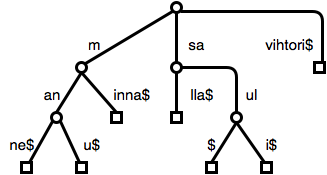
\includegraphics[scale=0.65]{CompactTrie}
\end{center}
\section*{Exercise 3}

\end{document}